\documentclass[tikz,border=20pt]{standalone}
\usetikzlibrary{calc,arrows.meta,positioning,shapes.geometric,fit}
\usepackage{amsmath,amssymb}

\begin{document}
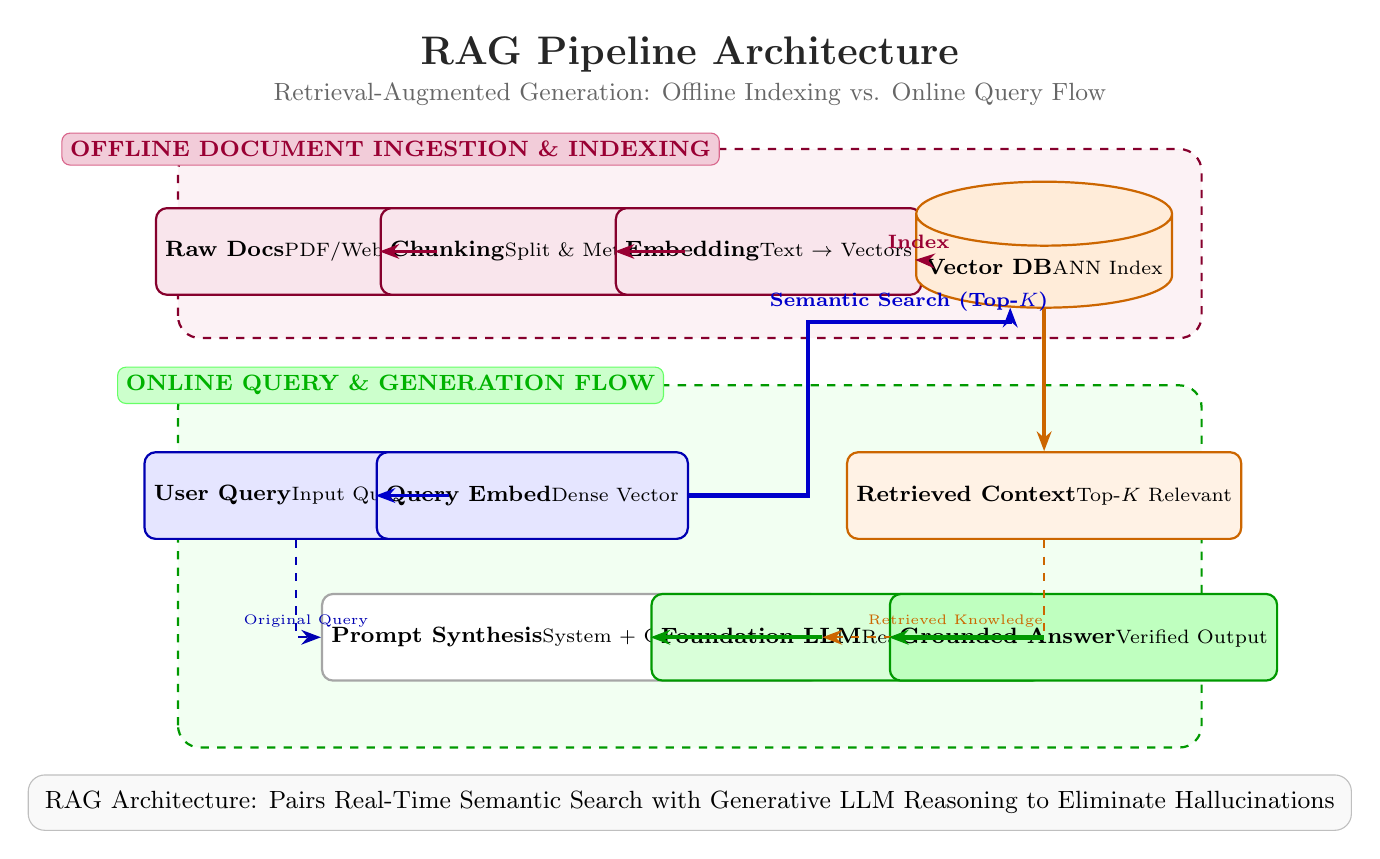
\begin{tikzpicture}[
  x=1cm, y=1cm, >=Stealth,
  proc/.style={rectangle, draw=blue!70!black, fill=blue!10, thick, rounded corners=4pt, text centered, minimum width=2.4cm, minimum height=1.1cm},
  purpleproc/.style={rectangle, draw=purple!70!black, fill=purple!10, thick, rounded corners=4pt, text centered, minimum width=2.4cm, minimum height=1.1cm},
  greenproc/.style={rectangle, draw=green!60!black, fill=green!15, thick, rounded corners=4pt, text centered, minimum width=2.4cm, minimum height=1.1cm},
  db/.style={cylinder, draw=orange!80!black, fill=orange!15, shape border rotate=90, aspect=0.25, thick, text centered, minimum width=2.2cm, minimum height=1.6cm},
  line/.style={draw, thick, -{Stealth[length=2.5mm]}}
]

  % Title
  \node[font=\bfseries\Large, text=black!85] at (6.0, 5.0) {RAG Pipeline Architecture};
  \node[font=\small, text=gray!80!black] at (6.0, 4.5) {Retrieval-Augmented Generation: Offline Indexing vs. Online Query Flow};

  % ==================== LANE 1: OFFLINE INGESTION (Top) ====================
  \draw[purple!70!black, thick, dashed, fill=purple!5, rounded corners=8pt] (-0.5, 1.4) rectangle (12.5, 3.8);
  \node[font=\bfseries\footnotesize, text=purple!80!black, fill=purple!20, draw=purple!60, rounded corners=3pt, inner sep=3pt] at (2.2, 3.8) {
    OFFLINE DOCUMENT INGESTION \& INDEXING
  };

  % 1. Raw Docs
  \node[purpleproc] (docs) at (1.0, 2.5) {\footnotesize \textbf{Raw Docs}\\ \scriptsize PDF/Web/DB};
  % 2. Chunking
  \node[purpleproc] (chunk) at (4.0, 2.5) {\footnotesize \textbf{Chunking}\\ \scriptsize Split \& Metadata};
  % 3. Embedding Model
  \node[purpleproc] (embed) at (7.0, 2.5) {\footnotesize \textbf{Embedding}\\ \scriptsize Text $\rightarrow$ Vectors};
  % 4. Vector DB (Cylinder)
  \node[db] (vdb) at (10.5, 2.3) {\footnotesize \textbf{Vector DB}\\ \scriptsize ANN Index};

  \draw[line, purple!80!black] (docs) -- (chunk);
  \draw[line, purple!80!black] (chunk) -- (embed);
  \draw[line, purple!80!black, line width=1.5pt] (embed) -- (vdb) node[midway, above, font=\scriptsize\bfseries] {Index};

  % ==================== LANE 2: ONLINE RETRIEVAL & GENERATION (Bottom) ====================
  \draw[green!60!black, thick, dashed, fill=green!5, rounded corners=8pt] (-0.5, -3.8) rectangle (12.5, 0.8);
  \node[font=\bfseries\footnotesize, text=green!70!black, fill=green!20, draw=green!60, rounded corners=3pt, inner sep=3pt] at (2.2, 0.8) {
    ONLINE QUERY \& GENERATION FLOW
  };

  % 1. User Query
  \node[proc] (query) at (1.0, -0.6) {\footnotesize \textbf{User Query}\\ \scriptsize Input Question};
  % 2. Query Embedding
  \node[proc] (qembed) at (4.0, -0.6) {\footnotesize \textbf{Query Embed}\\ \scriptsize Dense Vector};
  % 3. Retrieved Context
  \node[rectangle, draw=orange!80!black, fill=orange!10, thick, rounded corners=4pt, text centered, minimum width=2.4cm, minimum height=1.1cm] (context) at (10.5, -0.6) {
    \footnotesize \textbf{Retrieved Context}\\ \scriptsize Top-$K$ Relevant
  };

  % 4. Prompt Synthesis
  \node[rectangle, draw=gray!70, fill=white, thick, rounded corners=4pt, text centered, minimum width=2.6cm, minimum height=1.1cm] (synth) at (4.5, -2.4) {
    \footnotesize \textbf{Prompt Synthesis}\\ \scriptsize System + Context + Query
  };

  % 5. Foundation LLM
  \node[greenproc] (llm) at (8.0, -2.4) {\footnotesize \textbf{Foundation LLM}\\ \scriptsize Reasoning Engine};
  % 6. Grounded Answer
  \node[greenproc, fill=green!25] (answer) at (11.0, -2.4) {\footnotesize \textbf{Grounded Answer}\\ \scriptsize Verified Output};

  % Connectors within online flow
  \draw[line, blue!80!black] (query) -- (qembed);
  \draw[line, blue!80!black, line width=1.5pt] (qembed.east) -- (7.5, -0.6) -- (7.5, 1.6) -| (vdb.230)
    node[pos=0.25, above, font=\scriptsize\bfseries, text=blue!80!black] {Semantic Search (Top-$K$)};
  \draw[line, orange!80!black, line width=1.5pt] (vdb.south) -- (context.north);

  % User query down to synthesis
  \draw[line, blue!70!black, dashed] (query.south) |- (synth.west) node[pos=0.7, above, font=\tiny] {Original Query};
  % Context to synthesis
  \draw[line, orange!80!black, dashed] (context.south) |- (synth.east) node[pos=0.7, above, font=\tiny] {Retrieved Knowledge};

  % Synthesis to LLM to Answer
  \draw[line, green!60!black, line width=1.5pt] (synth) -- (llm);
  \draw[line, green!60!black, line width=2pt] (llm) -- (answer);

  % Bottom Summary Box
  \node[draw=gray!50, fill=gray!5, rounded corners=6pt, font=\small, inner sep=6pt] at (6.0, -4.5) {
    RAG Architecture: Pairs Real-Time Semantic Search with Generative LLM Reasoning to Eliminate Hallucinations
  };

\end{tikzpicture}
\end{document}
